L'introduction est une section requise dans un rapport technique. Introduisez votre travail, l'idée de départ et les objectifs attendus. Un lecteur qui découvrirait votre projet au travers de cette introduction devrait ainsi être capable d'en comprendre le cadre, l'idée générale et les aboutissants du projet.

Le but de ce projet de bachelor consiste, premièrement, d'apporter plus de sécurité au système de pinces optiques par laser afin de faciliter son utilisation au quotidien. Deuxièmement, une proposition d'expérience avec un mode d'emploi compact est proposé pour le cours de NANO pour les systèmes industriels.Troisièmement, des tests de déplacements de microbilles dans différents milieux, de différentes viscosités, dans différents types de réservoirs ainsi que de multiples canaux.

\section{Contexte}
Cette section \underline{n'est pas obligatoire}, mais elle est souvent présente dans un rapport technique pour compléter l'introduction et définir le contexte du travail \cad le cadre formel dans lequel le travail est mené. (A PEUT ETRE COMPLETER)
\newline\newline
Le kit de pinces optiques portables, Portable Optical Tweezers, est conçu par l'entreprise Thorlabs. Thorlabs est une entreprise américaine qui conçoit des composants optiques, des lasers, des instruments de mesure. (A PEUT ETRE COMPLETER)
\newline\newline
La figure ci-dessous (voir Figure \ref{kit vierge}) correspond au kit reçu lors du premier jour de TB. Le kit a été monté par un assistant du laboratoire COMATEC-LANS. sakut

\begin{figure}[H]
    \begin{center}
        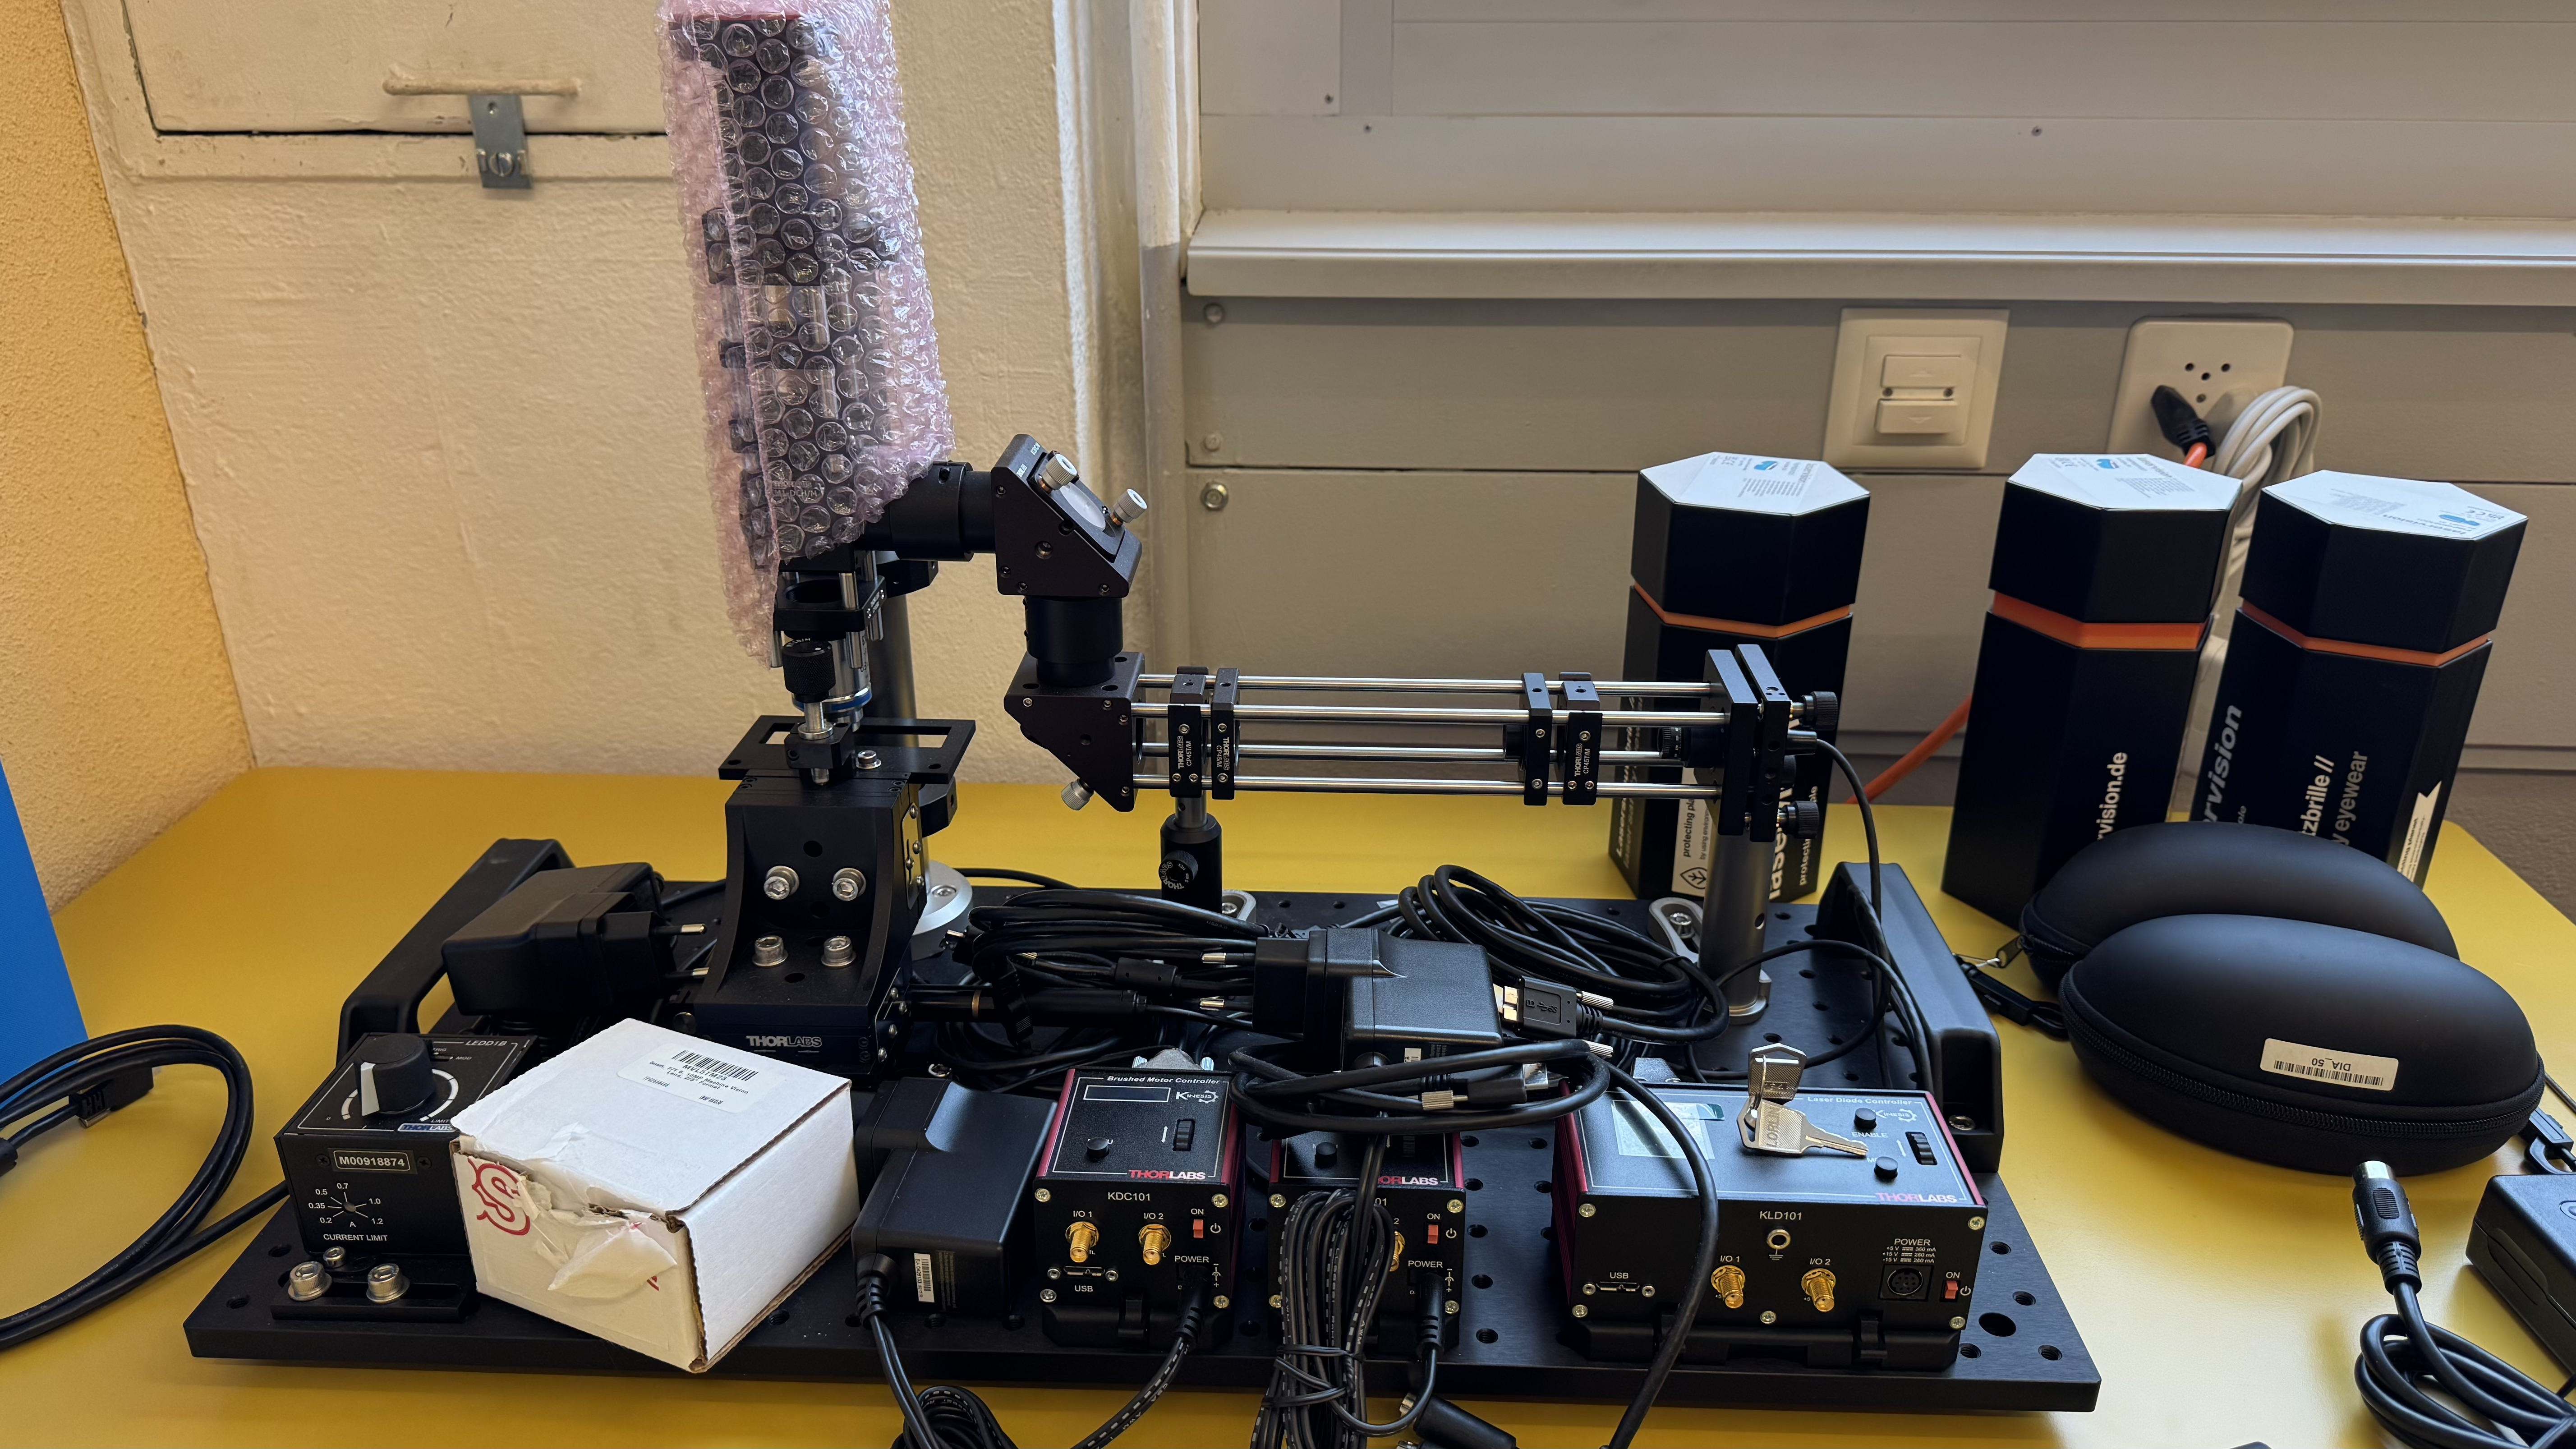
\includegraphics[width=0.7\textwidth]{assets/figures/kit_vierge.jpeg}
    \end{center}
    \caption{kit Portable Optical Tweezers de Thorlabs}
    \label{kit vierge}
\end{figure}


















%%if
\section{Citations et bibliographie}
Citer vos sources est essentiel. Avec \texttt{biblatex} vous pouvez facilement citer des articles, des livres ou des sites internet. Toutes les citations dans le texte seront automatiquement regroupées en fin de document dans la section \guillemotleft Bibliographie\guillemotright. Par exemple, citons un article d'Einstein \cite{einstein} ou le livre de Dirac \cite{dirac}.

Parfois il peut être utile d'utiliser un gestionnaire de bibliographie. La communauté académique recommande l'outil \href{https://www.zotero.org/}{Zotero} qui permet de gérer une bibliothèque numérique d'ouvrages et de références numériques. Il permet également de générer une bibliographie compatible avec \LaTeX.

Notez qu'il est très facile d'obtenir l'extrait \texttt{bibtex} depuis des journaux. Sélectionnez \emph{export/citation}. Si vous le pouvez choisissez \texttt{bibtex}. Dans le cas d'un format \texttt{.ris}, utilisez un convertisseur en ligne comme \href{http://www.bruot.org/ris2bib/}{ris2bib}.

\section{Adapter votre modèle}
Ce document n'est qu'un modèle ayant pour but de revoir les quelques avantages de \LaTeX~ et les fonctionnalités qui pourraient vous être utiles pour rédiger un rapport académique. N'hésitez pas à supprimer les parties inutiles et à adapter ce modèle à vos besoins.
%%fi